\chapter{Propiedaes térmicas reticulares} \label{Ch:05}

En este Tema se estudia la parte más \textit{física} de las vibraciones atómicas en los sólidos. En concreto, veremos cómo se pueden entender desde la dinámica de red propiedades como \textit{calor específico}, la \textit{conductividad térmica} y la \textit{dilatación térmica} de los sólidos.

\section{Densidad de modos}

\subsection{Condiciones de contorno}

\begin{figure}[h!] \centering
    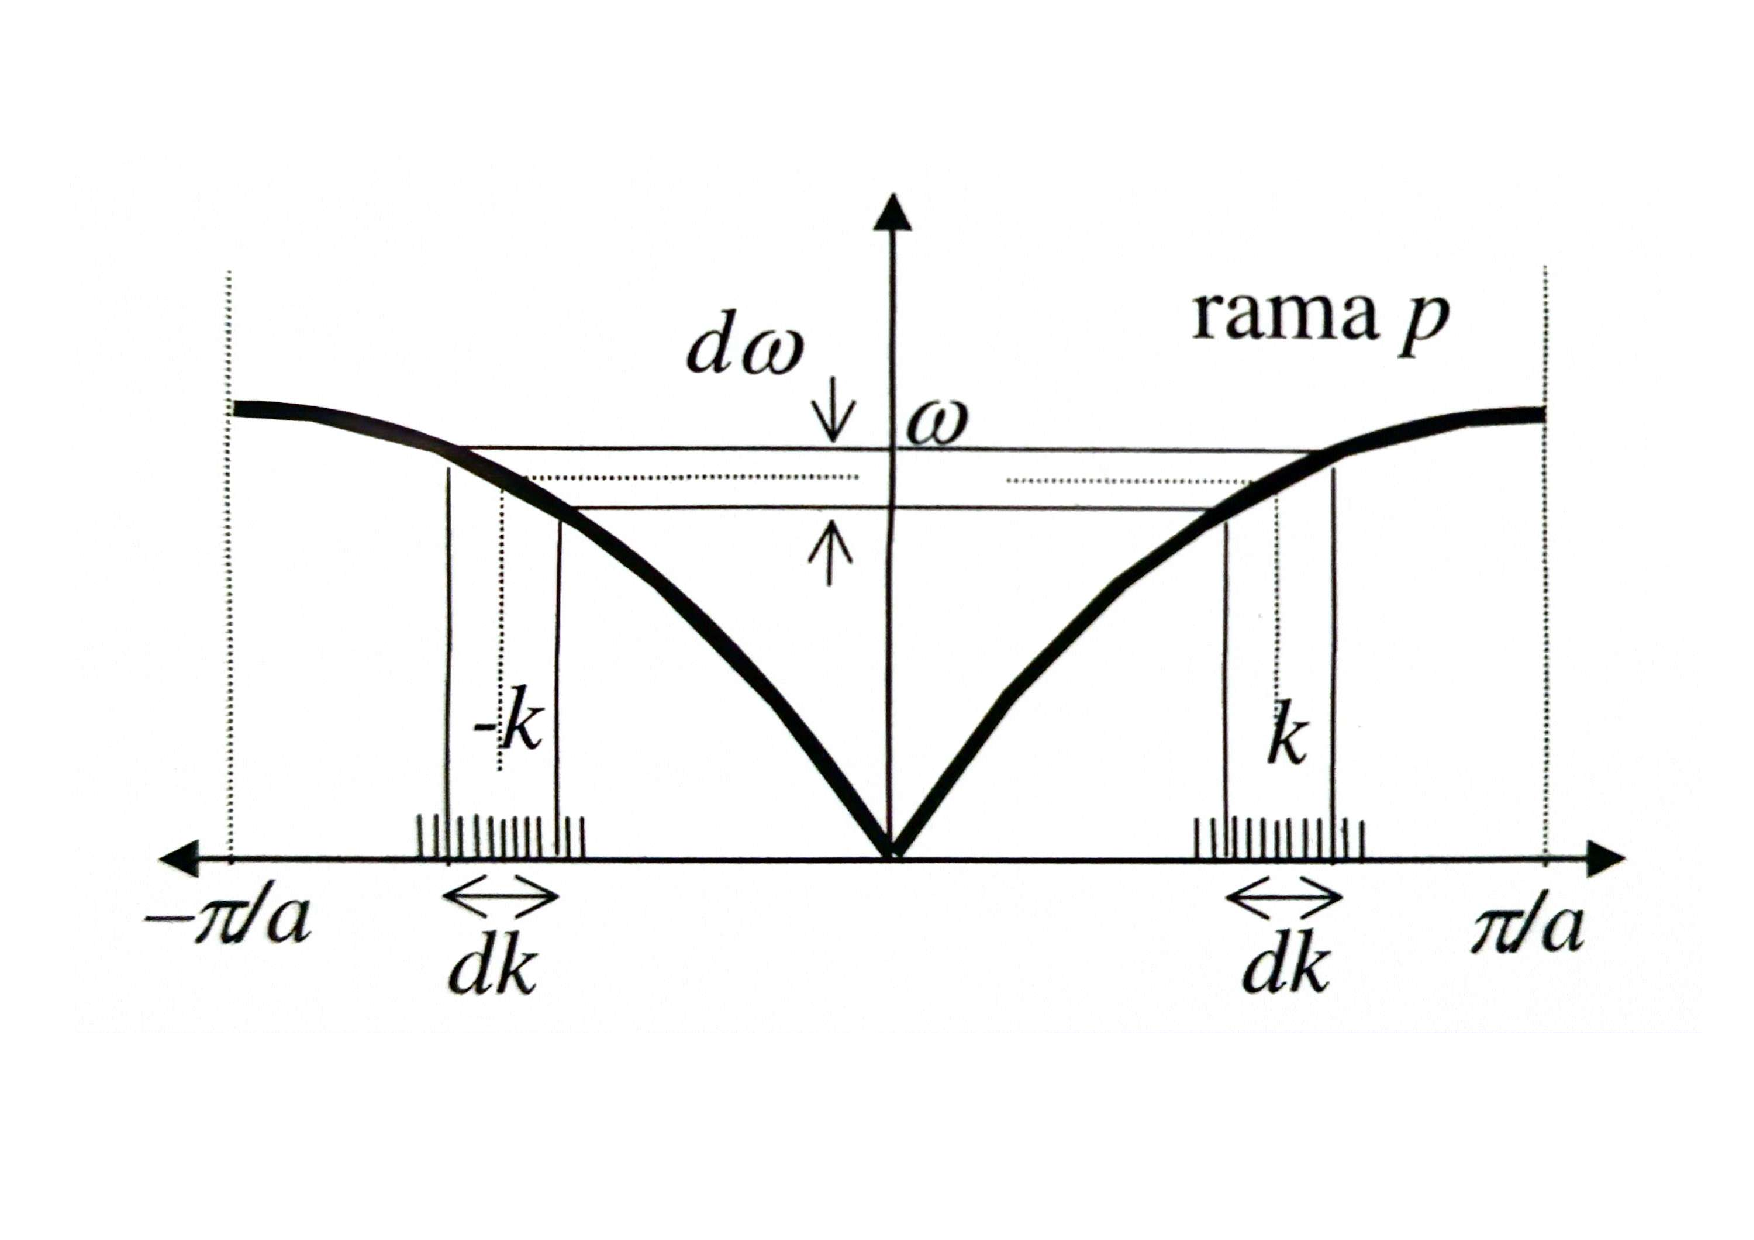
\includegraphics[scale=0.5]{Cuerpo/Ch_05/Fotos libro 1.pdf}
    \caption{Relación de dispersión para una cadena monoatómica. Equivalencia entre la densidad de modos en $k$ y en $\omega$.}
    \label{Fig:05-01}
\end{figure}    


\subsection{Cálculo de la densidad de modo}

\subsection{Aproximación de Debye}

\begin{figure}[h!] \centering
    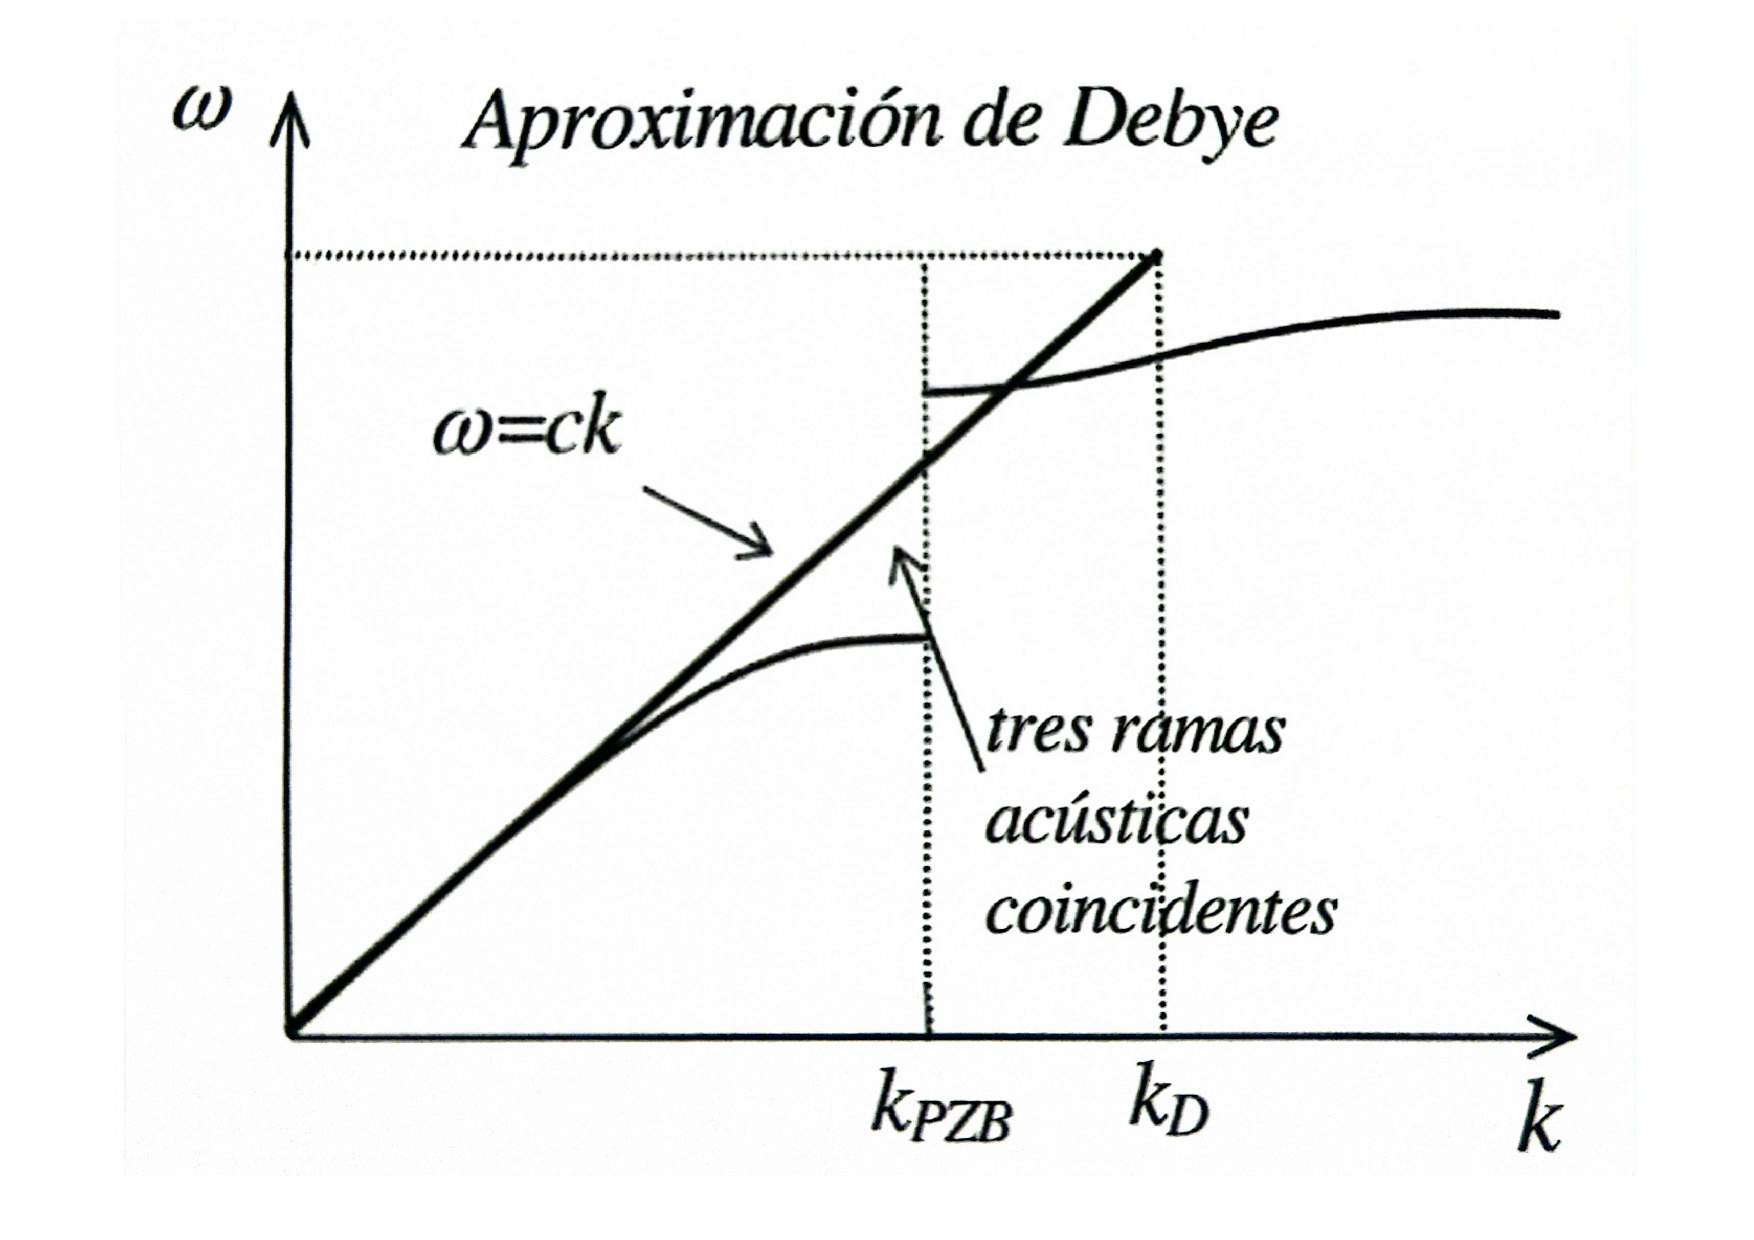
\includegraphics[scale=0.5]{Cuerpo/Ch_05/Fotos libro 2.pdf}
    \caption{Representación de la aproximación de Debye. Todas las ramas se sustituyen por tres acústicas degeneradas.}
    \label{Fig:05-02}
\end{figure}    


\section{Capacidad térmica reticular}

\subsection{Estadística de fonones}

\begin{figure}[h!] \centering
    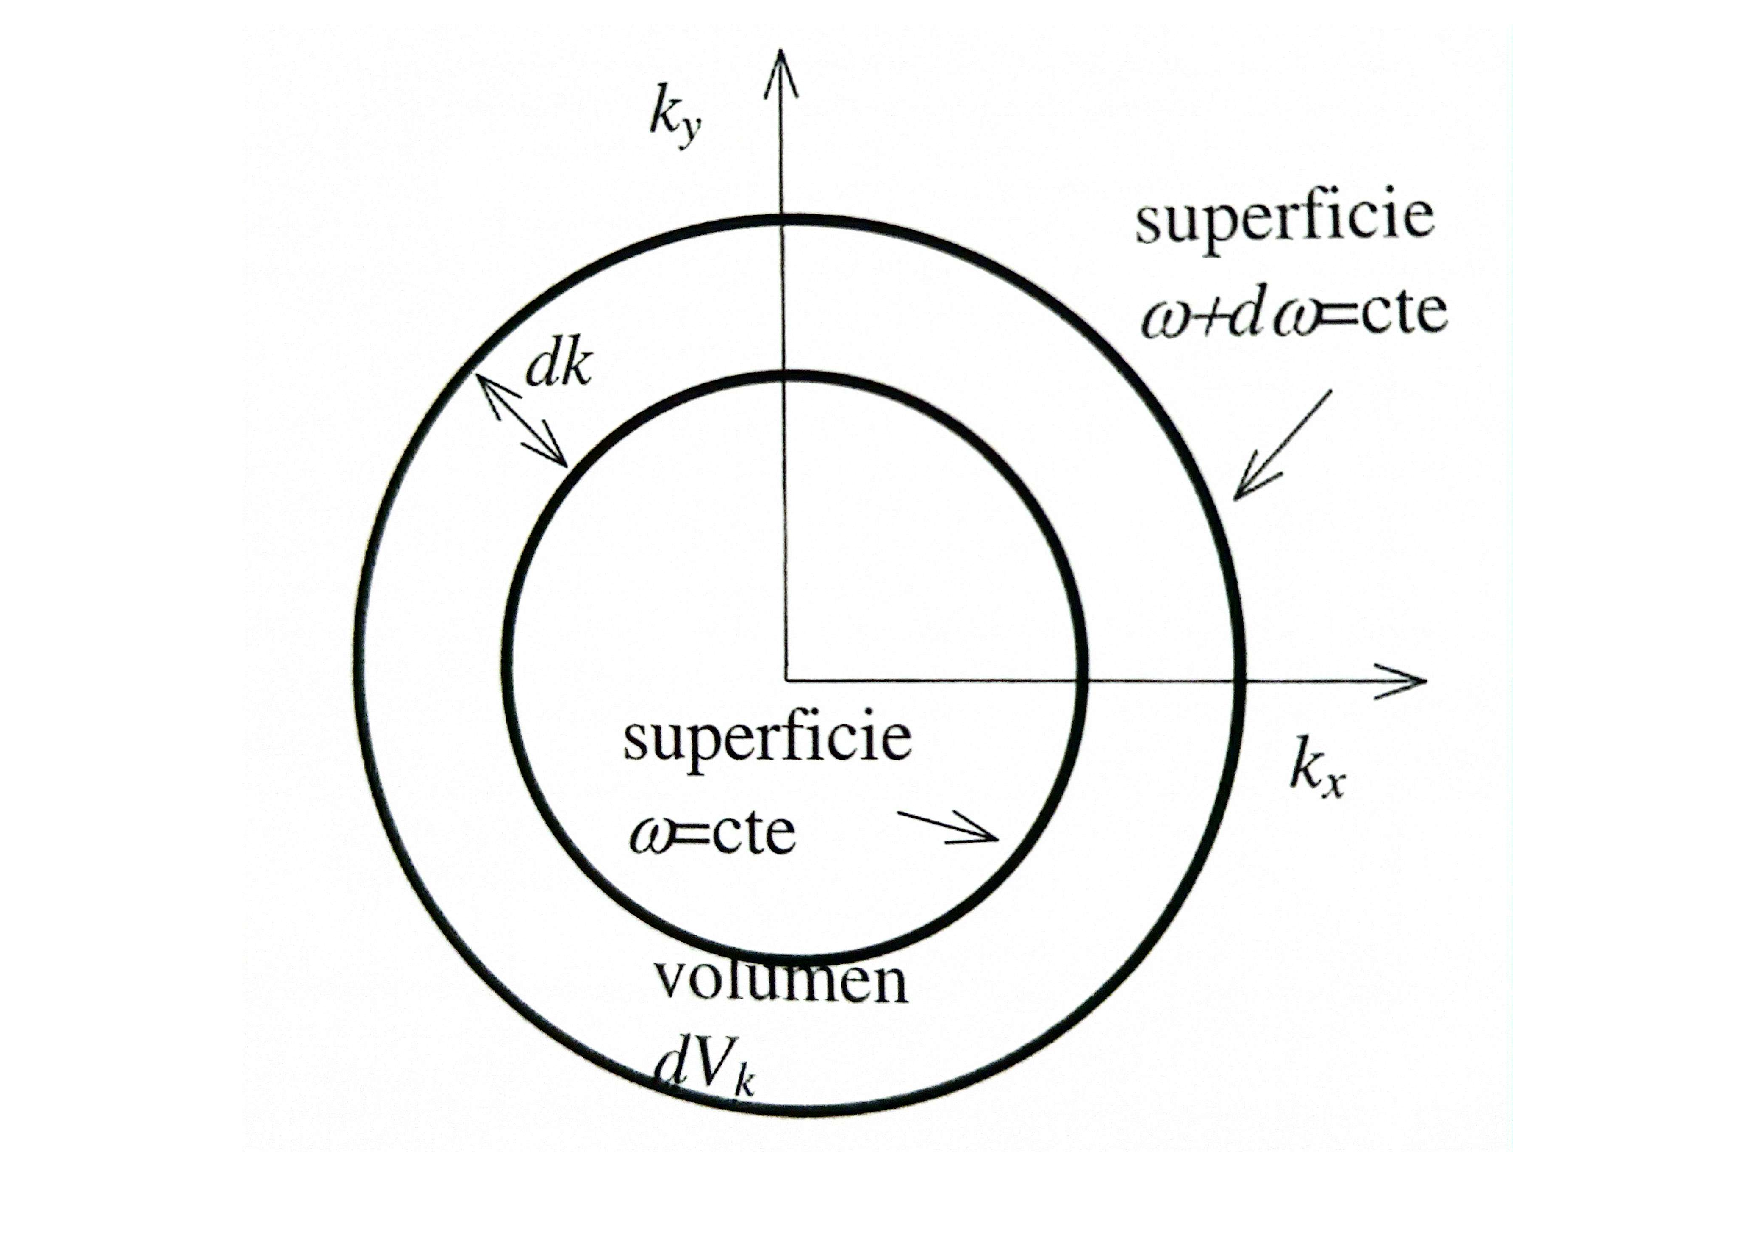
\includegraphics[scale=0.5]{Cuerpo/Ch_05/Fotos libro 3.pdf}
    \caption{Sección de una superficie de frecuencia constante en la aproximación de Debye.}
    \label{Fig:05-03}
\end{figure}    


\subsection{Cálculo de la capacidad térmica}

\begin{figure}[h!] \centering
    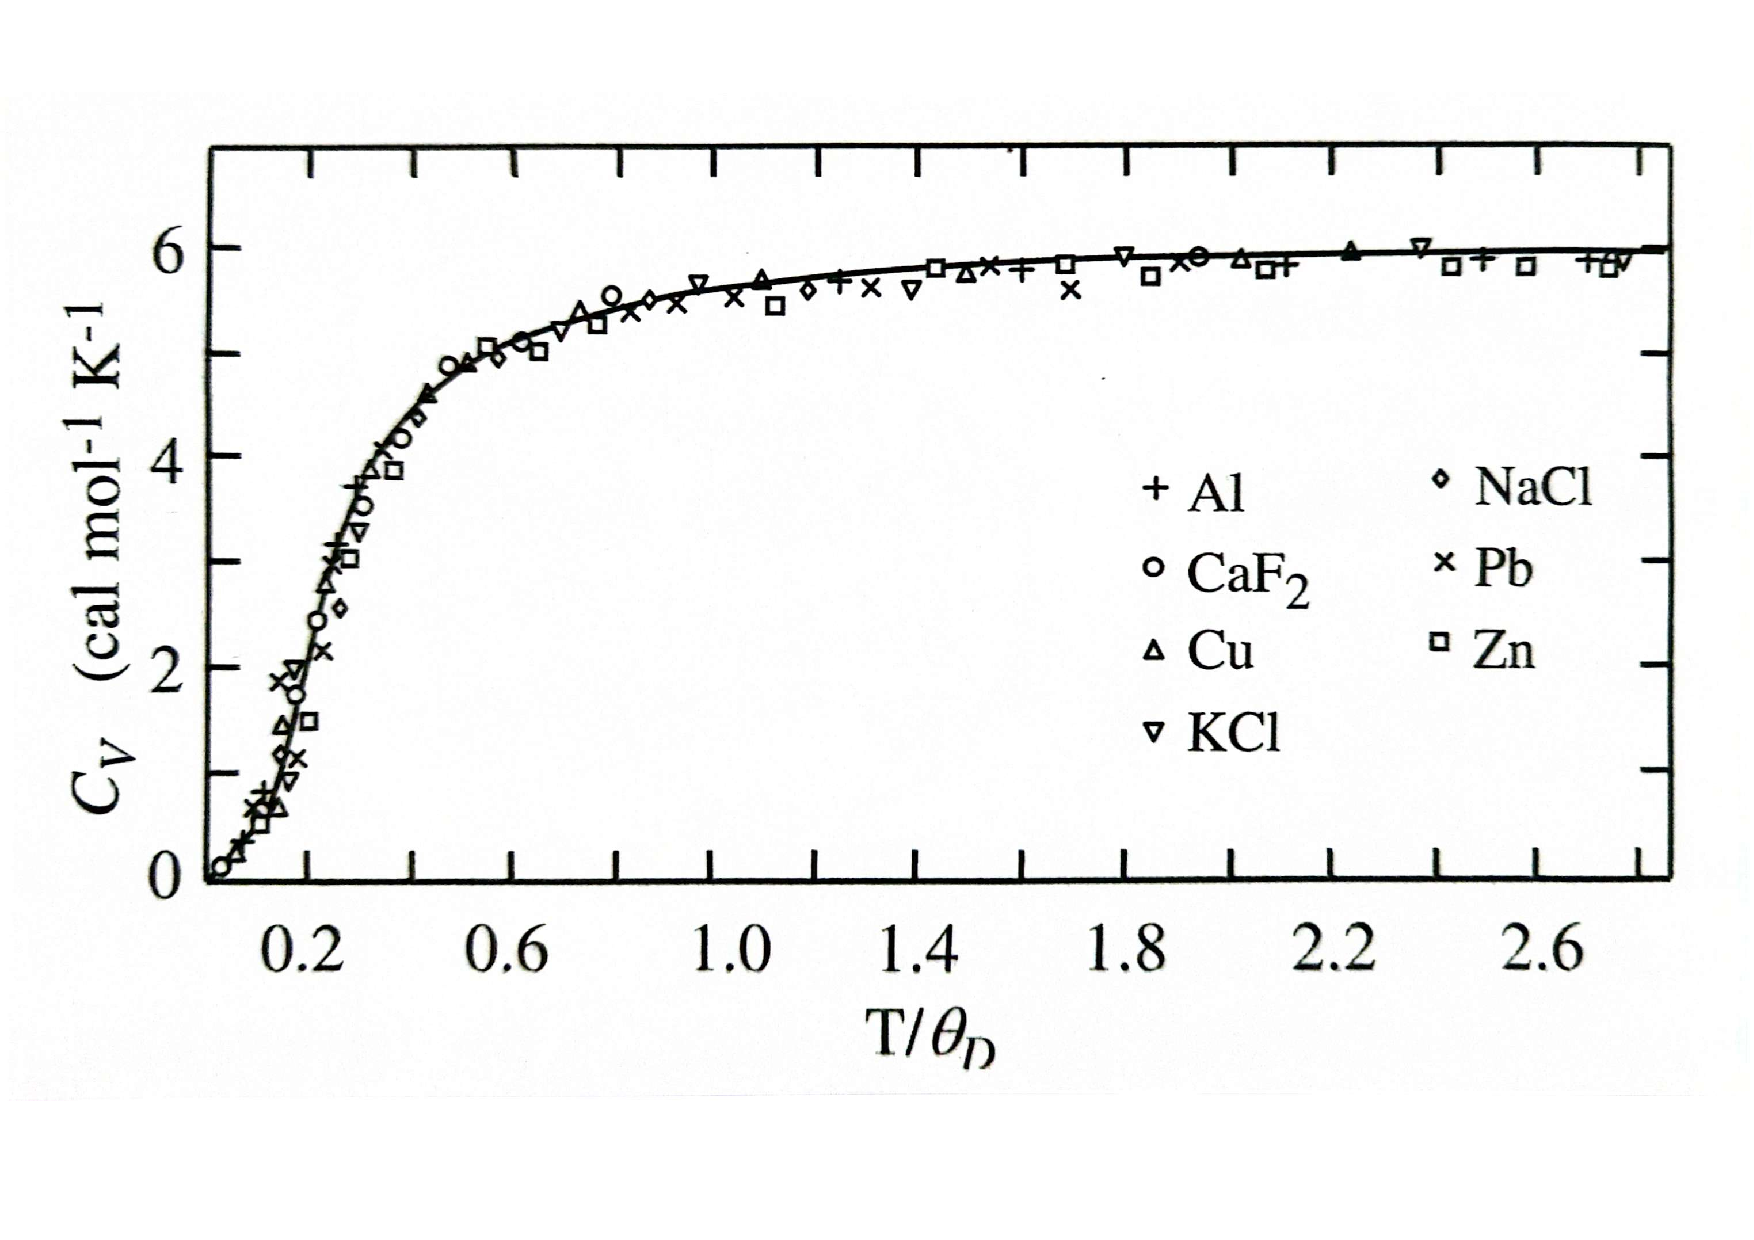
\includegraphics[scale=0.5]{Cuerpo/Ch_05/Fotos libro 4.pdf}
    \caption{Capacidad térmica por mol frente $T/\theta_D$ para diversos tipos de cristales.}
    \label{Fig:05-04}
\end{figure}    



\section{Efectos anarmónicos}

\subsection{Dilatación térmica}

\begin{figure}[h!] \centering
    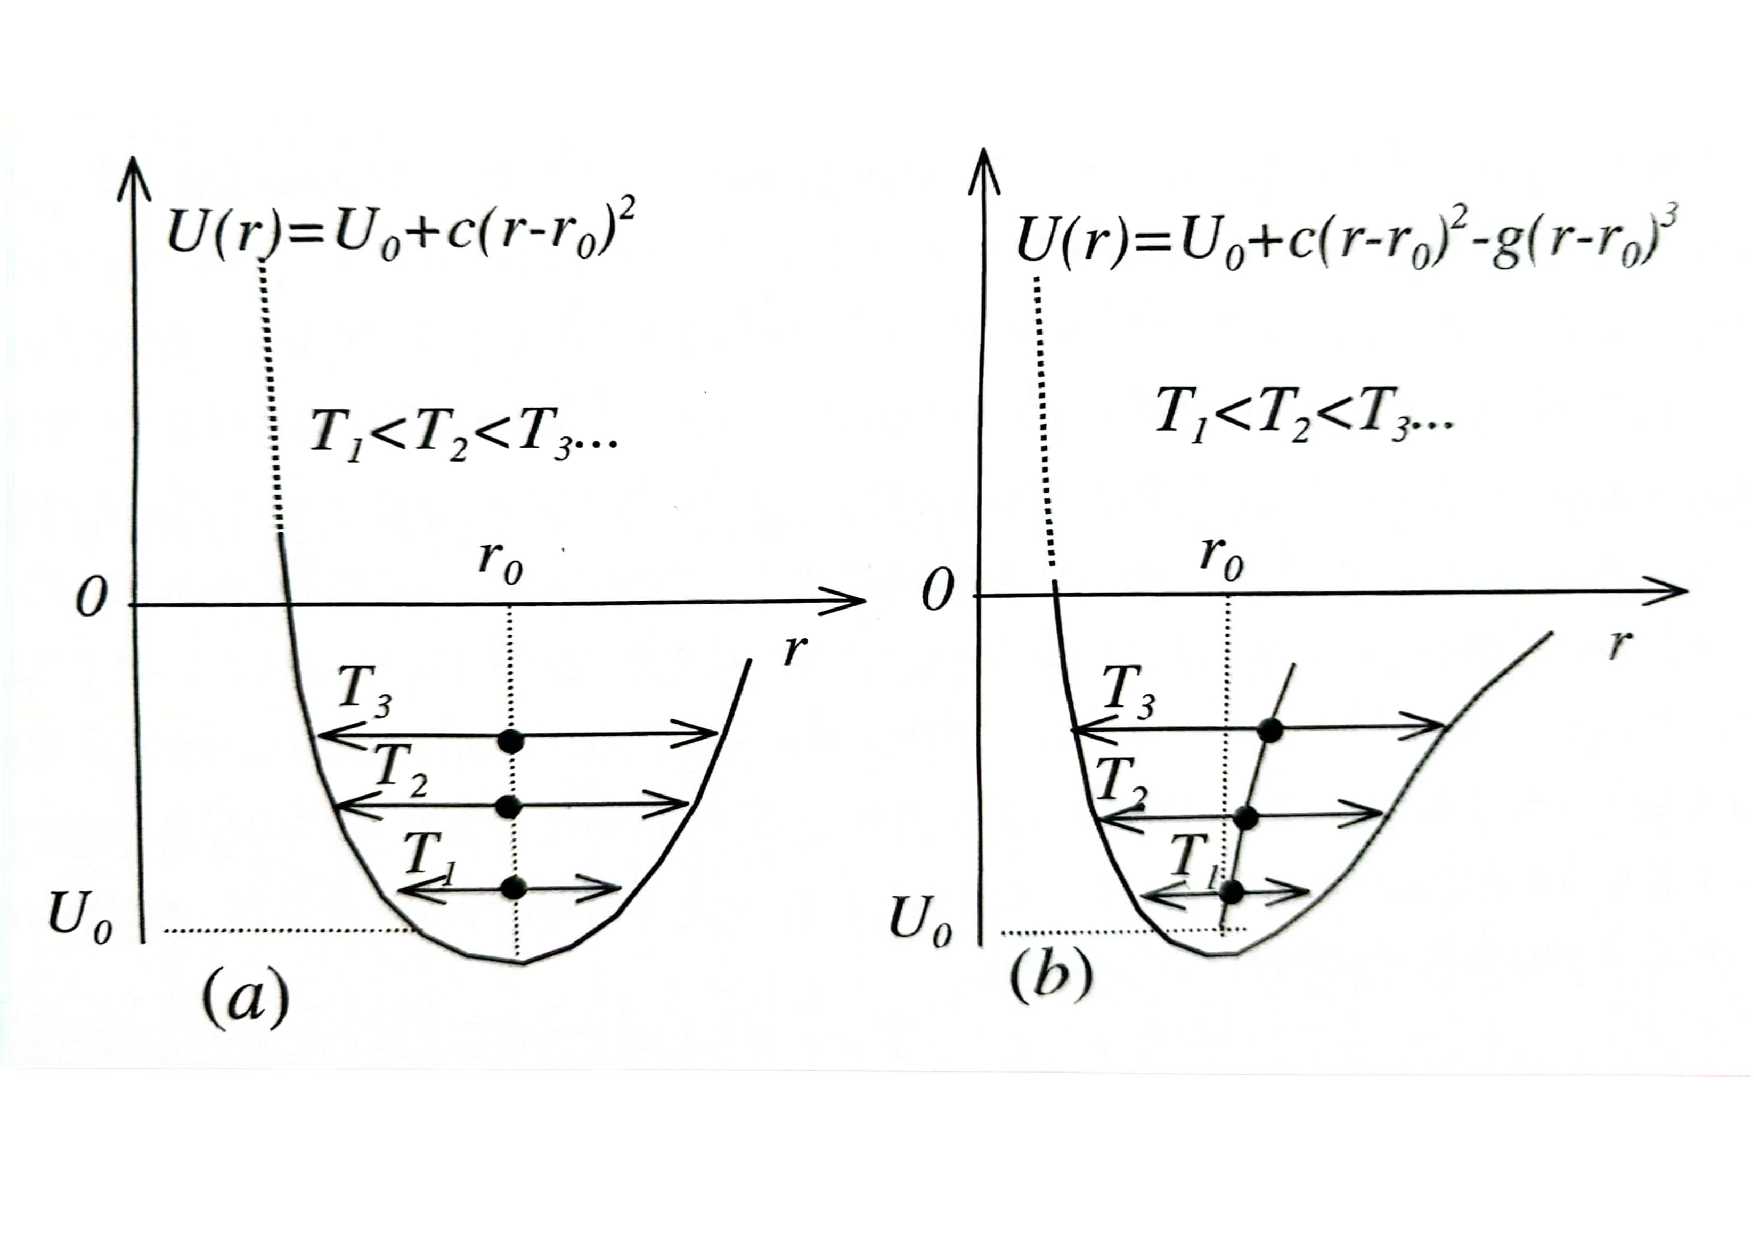
\includegraphics[scale=0.5]{Cuerpo/Ch_05/Fotos libro 5.pdf}
    \caption{Potencial por par de átomos según la aproximación armónica (a) y según la aproximación anarmónica (b) que permite explicar de los cristales cuando se calientan.}
    \label{Fig:05-05}
\end{figure}    


\subsection{Conductividad térmica}

\begin{figure}[h!] \centering
    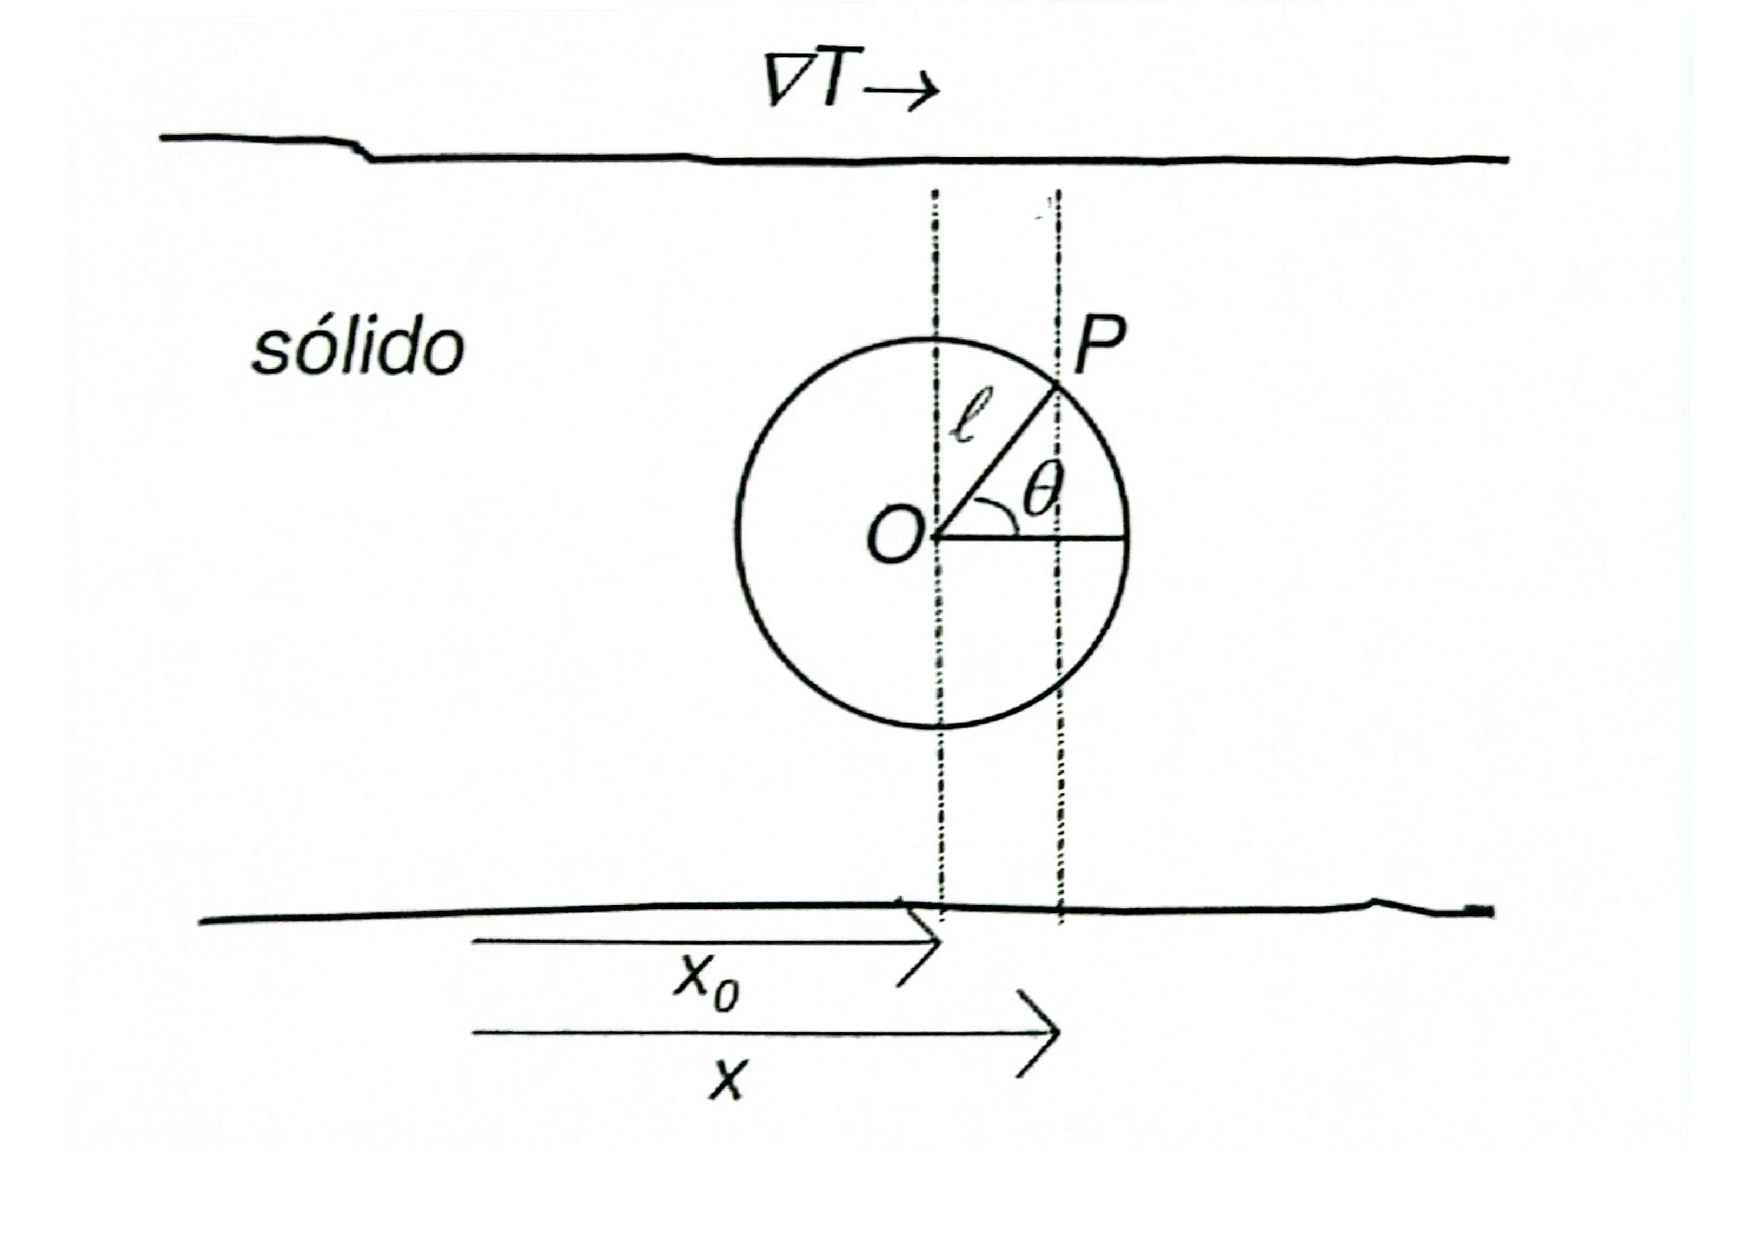
\includegraphics[scale=0.5]{Cuerpo/Ch_05/Fotos libro 6.pdf}
    \caption{Transporte de calor mediante fonones en presencia de un gradiente uniforme de temperatura. La corriente térmica en $O$ se debe a los fonones que, en media, han sufrido la última colisión en un punto $P$ a distancia $l=c\tau$.}
    \label{Fig:05-06}
\end{figure}    
\begin{figure}[h!] \centering
    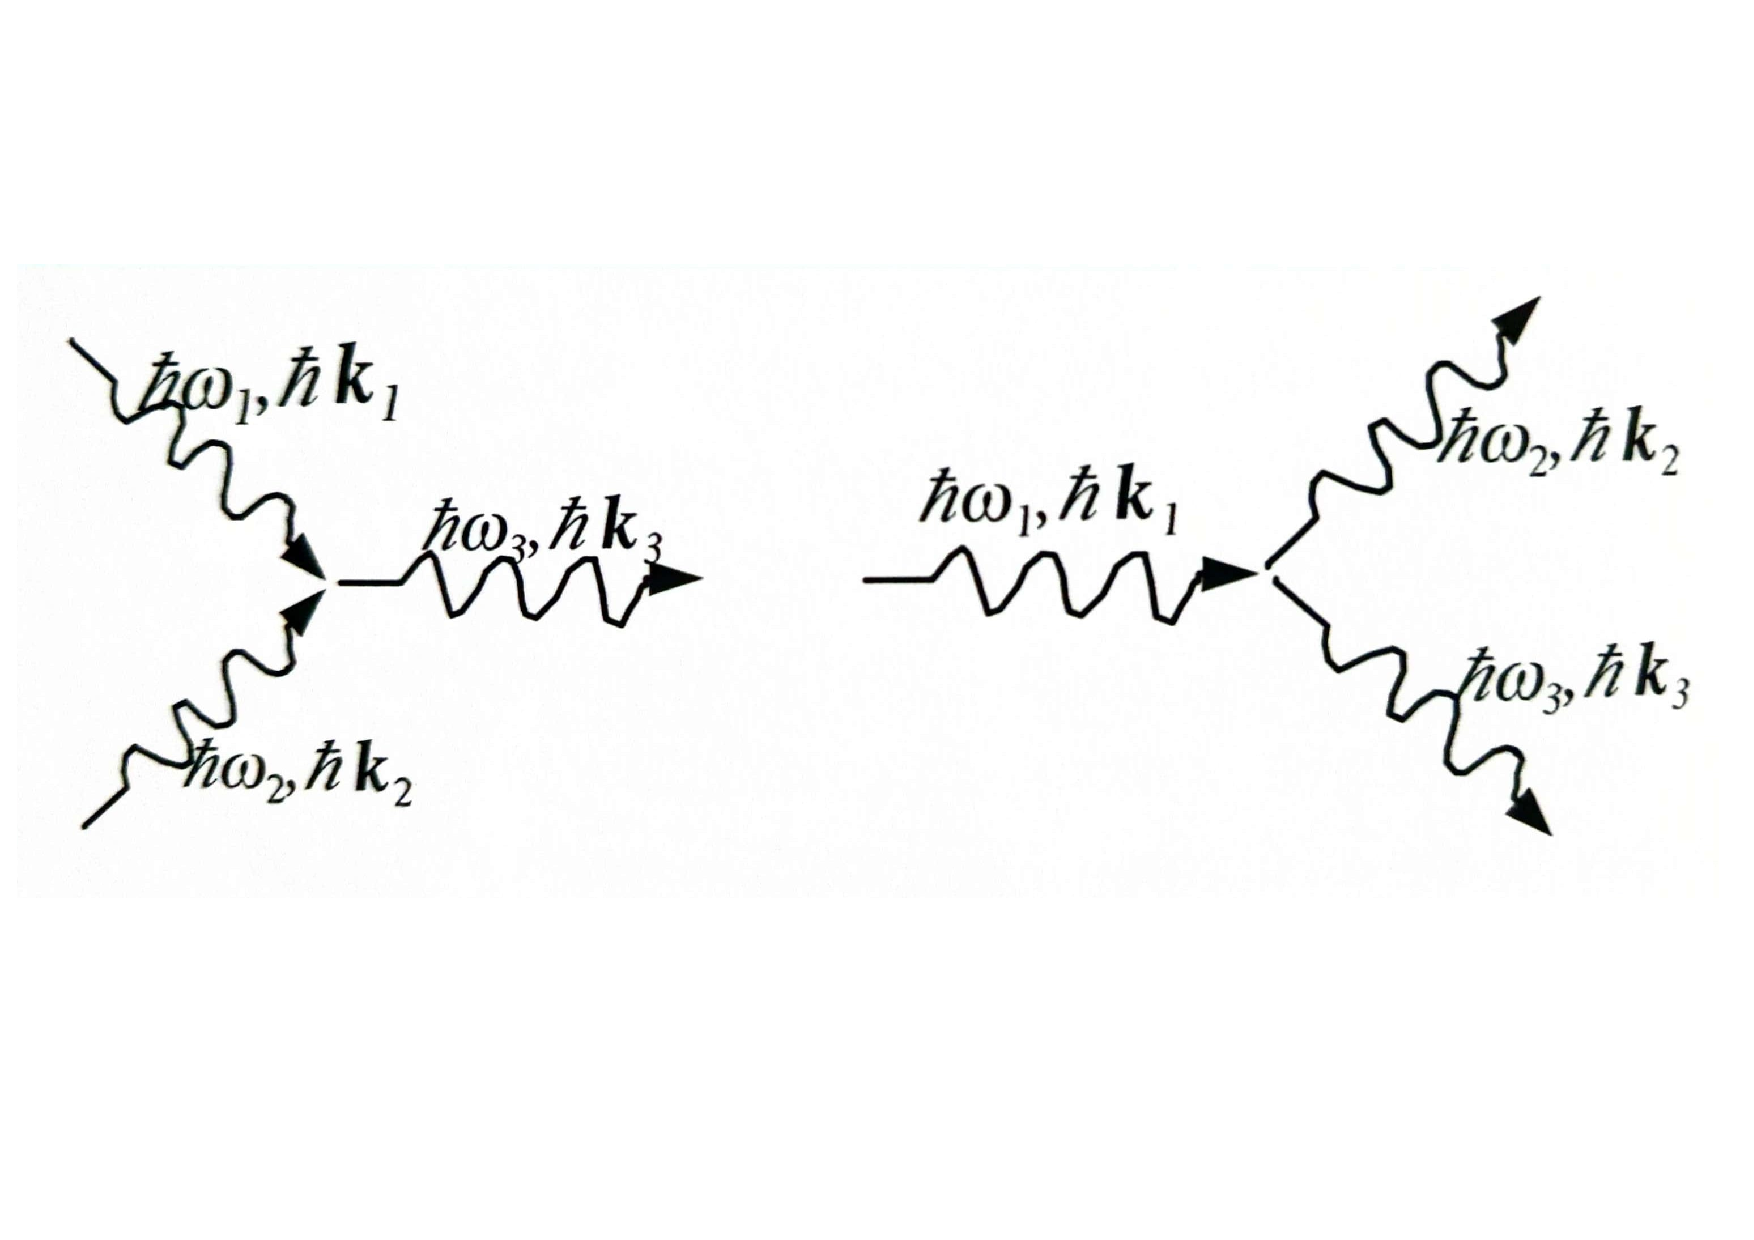
\includegraphics[scale=0.5]{Cuerpo/Ch_05/Fotos libro 7.pdf}
    \caption{Procesos de interacción entre fonones debidos a los términos (\textit{cúbicos}) anarmónicos del potencial de interacción entre átomos. Izquierda: Dos fonones interaccionan dando lugar a un tercer fonón. Derecha: Un fonón \textit{se rompe} en dos.}
    \label{Fig:05-07}
\end{figure}    
\begin{figure}[h!] \centering
    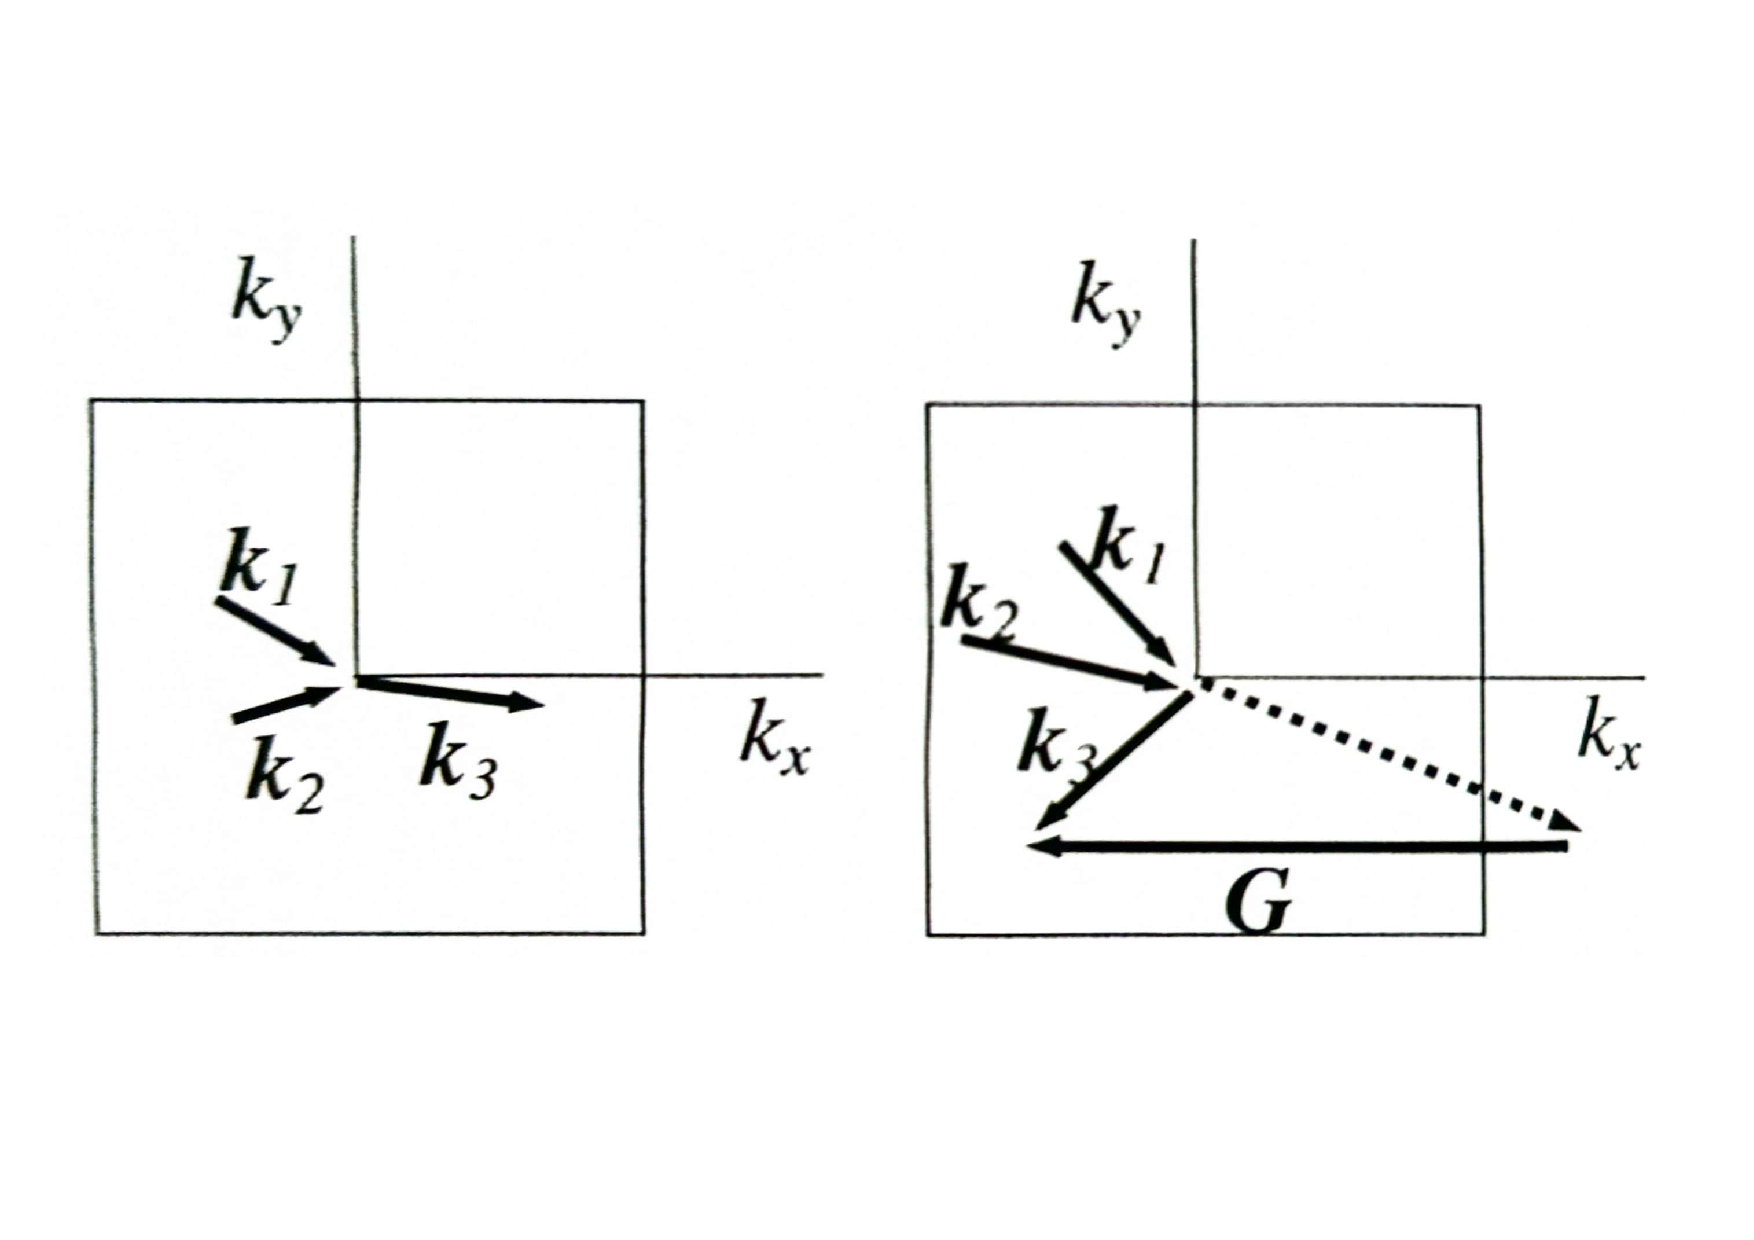
\includegraphics[scale=0.5]{Cuerpo/Ch_05/Fotos libro 8.pdf}
    \caption{Izquierda: Proceso $N$ que no degrada el transporte de energía térmica. Derecha: Proceso $U$ que degrada fuertemente el transporte de calor.}
    \label{Fig:05-08}
\end{figure}    
\begin{figure}[h!] \centering
    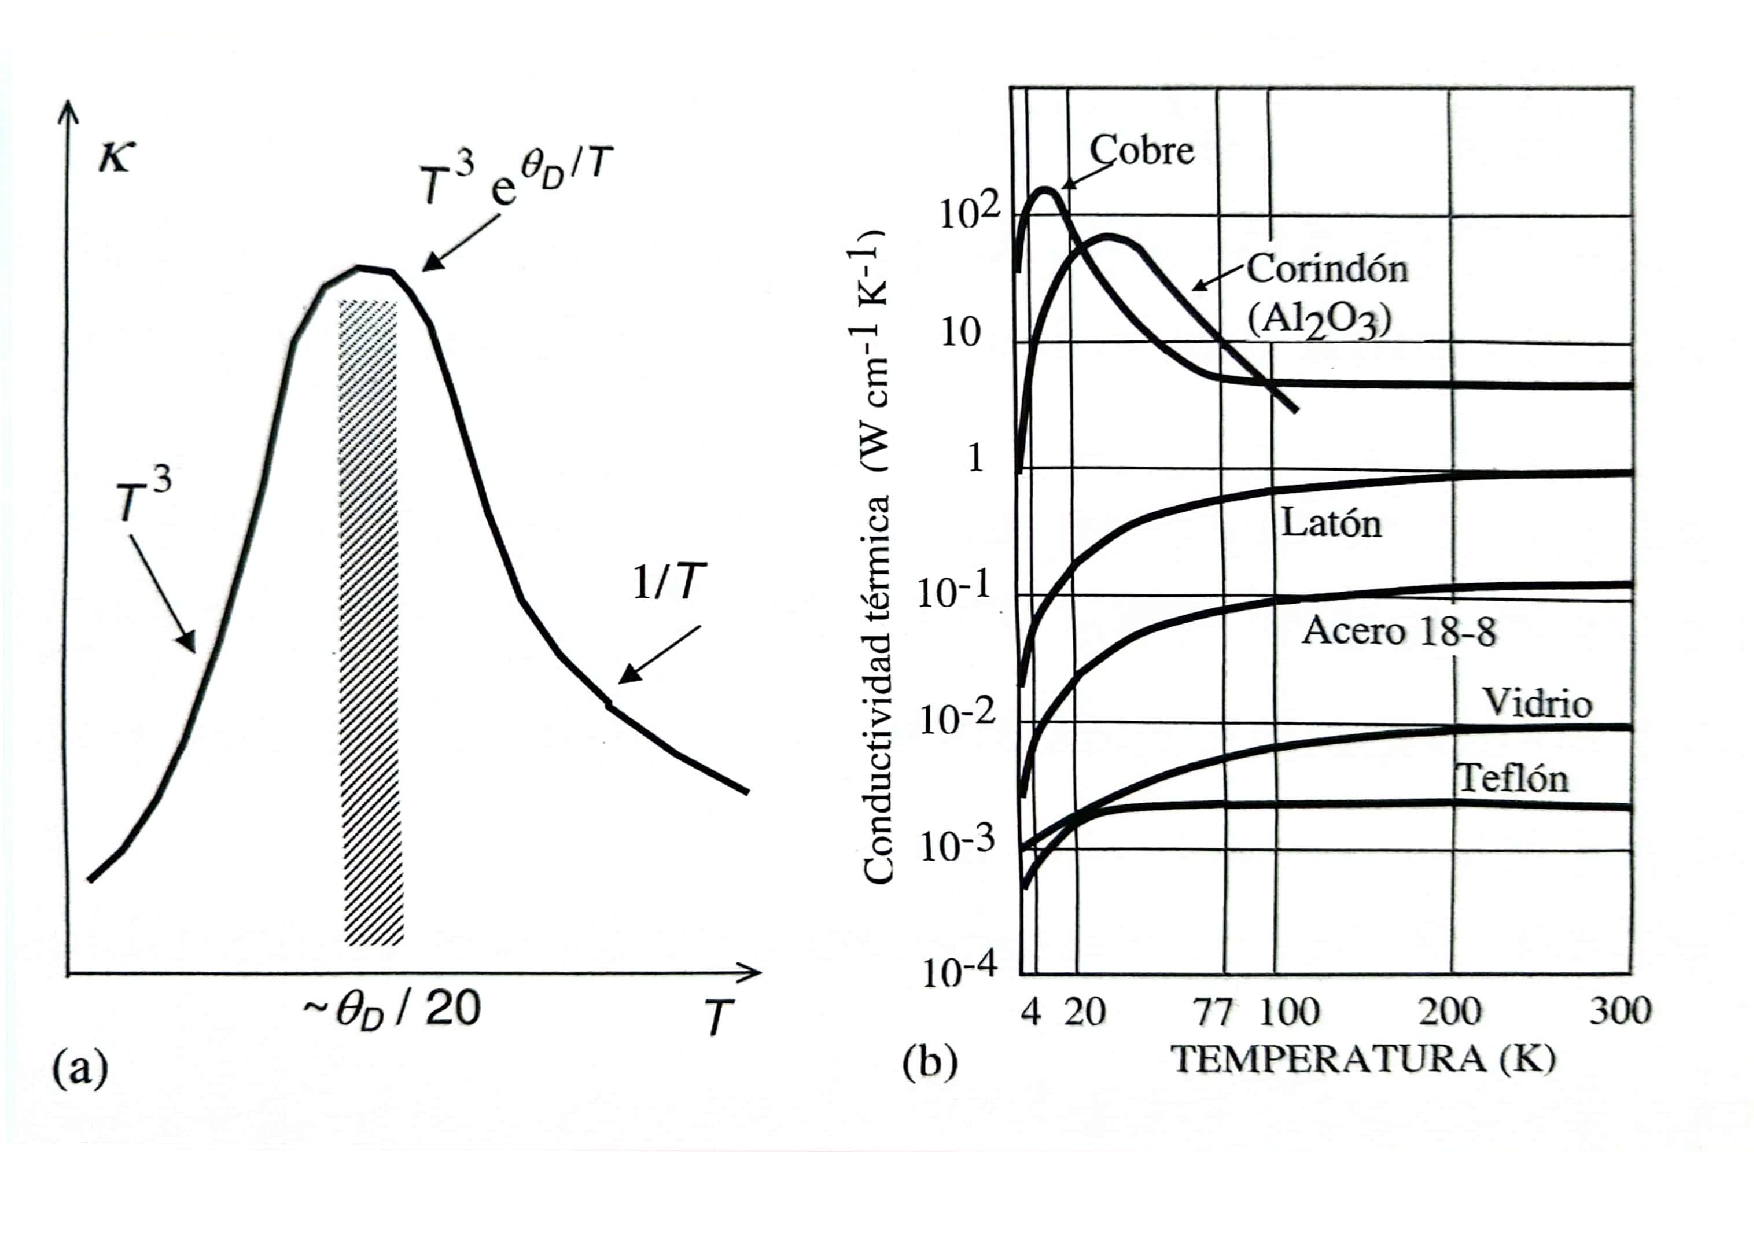
\includegraphics[scale=0.5]{Cuerpo/Ch_05/Fotos libro 9.pdf}
    \caption{(a) Dependencia genérica de la conductividad térmica de los cristales con la temperatura. (b) Conductividad térmica frente a la temperatura para diversos tipos de sólidos.}
    \label{Fig:05-09}
\end{figure}    

